\subsubsection{Logitech C910}
\begin{figure}[H]
  \centering
  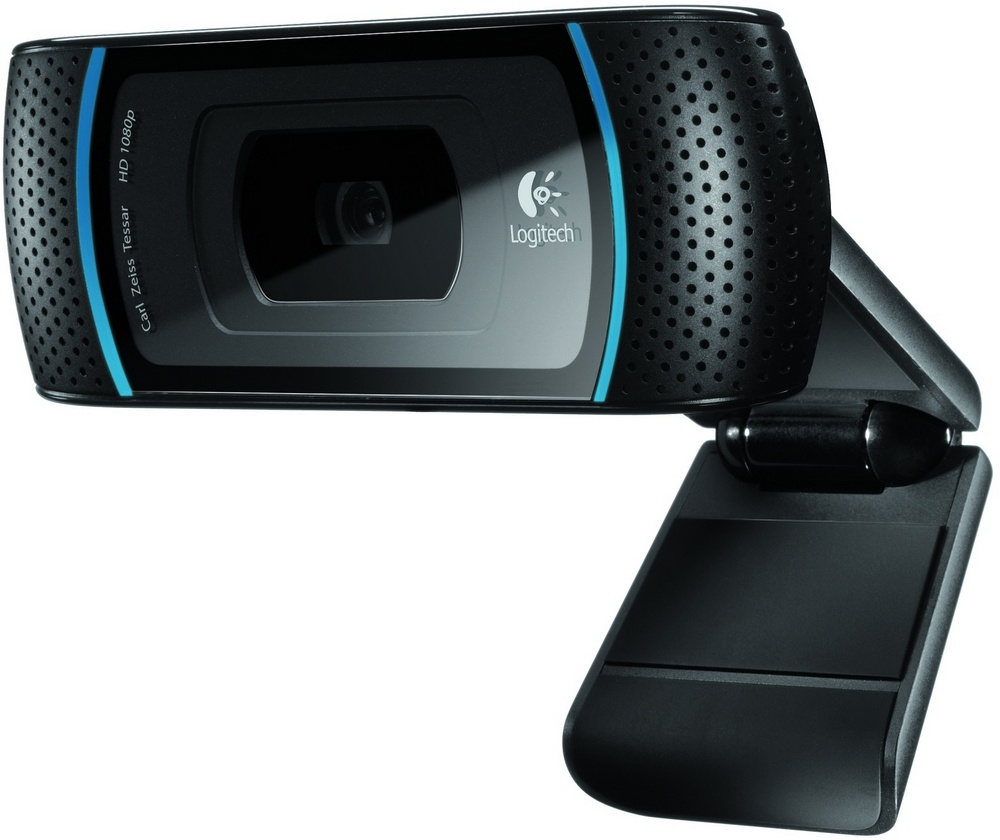
\includegraphics[width=3cm]{images/techAnalysis/LogitechC910.jpg}
  \caption{Logitech C910 camera \cite{Logitech-figure-C910}}\label{fig:sssec:LogitechC910}
\end{figure}
The Logitech C910, shown on \autoref{fig:sssec:LogitechC910}, is a 5MP camera with autofocus, with an 83 degree diagonal field of view.
It captures video at either 4:3 format up to 1600x1200 pixels, or 16:9 format at up to 1920x1080 pixels.
It connects to a computer through its USB cable and can be tilted 180 degrees vertically.
The camera also features a built-in stereo microphone which allows it to capture audio.
\cite{logitech_logitech_spec}
